\documentclass[11pt,a4paper,ngerman]{article}
\usepackage[bottom=2.5cm,top=2.5cm]{geometry} 
\usepackage{babel}
\usepackage[utf8]{inputenc} 
\usepackage[T1]{fontenc} 
\usepackage{ae} 
\usepackage{amssymb} 
\usepackage{amsmath} 
\usepackage{graphicx}
\usepackage{fancyhdr}
\usepackage{fancyref}
\usepackage{listings}
\usepackage{xcolor}
\usepackage{paralist}
\usepackage{subfigure}

%\usepackage[pdftex, bookmarks=false, pdfstartview={FitH}, linkbordercolor=white]{hyperref}
\usepackage{fancyhdr}
\pagestyle{fancy}
\fancyhead[C]{CoMa II}
\fancyhead[L]{Übung Nr. 8}
\fancyhead[R]{SoSe 2012}
\fancyfoot{}
\fancyfoot[L]{}
\fancyfoot[C]{\thepage / \pageref{LastPage}}
\renewcommand{\footrulewidth}{0.5pt}
\renewcommand{\headrulewidth}{0.5pt}
\setlength{\parindent}{0pt} 
\setlength{\headheight}{0pt}

\author{Tutor: Sebastian Scherer}
\date{}
\title{Max Wisniewski , Alexander Steen}

\begin{document}

\lstset{language=Pascal, basicstyle=\ttfamily\fontsize{10pt}{10pt}\selectfont\upshape, commentstyle=\rmfamily\itshape\small, keywordstyle=\rmfamily\bfseries, breaklines=true, frame=single, xleftmargin=3mm, xrightmargin=3mm, tabsize=2}

\maketitle
\thispagestyle{fancy}


%% ------------------------------------------------------
%%                     AUFGABE 1
%% ------------------------------------------------------

\section*{Aufgabe 1}
\begin{enumerate}[a)]
\item Verifizieren Sie, dass die Entwicklung der Wassertemperatur $\Theta(t)$ durch folgendes AWP modelliert wird
$$ \Theta'(t) = \frac{f}{V_0}(\Theta_1 - \Theta(t)), \quad \Theta(0) = \Theta_0$$ 

Sei $\Delta t > 0$, dann ist $\Theta(t + \Delta t) = \Theta(t) + \Delta \Theta$, wobei $\Delta \Theta$ die Temperaturänderung von $t$ bis $t + \Delta t$ bezeichnet.

Die Menge des zugelaufenen und abgelaufenen Wassers nach $\Delta t$ vergangener Zeit beträgt jeweils $\Delta t f$. Dann ist $\frac{1}{V_0}(\Delta t f \Theta_1 - \Delta t f \Theta(t))$ der gewichtete Durchschnitt (Temperaturdifferenz verteilt auf das Volumen) der Temperaturunterschiede und damit die Temperaturdifferenz $\Delta \Theta$. Also ist $\Theta(t + \Delta t) = \Theta(t) + \frac{1}{V_0}(\Delta t f \Theta_1 - \Delta t f \Theta(t)) = \Delta t \frac{f}{V_0} (\Theta_1 - \Theta(t))$.

Durch Umstellen erhalten wir $\frac{\Theta(t + \Delta t) - \Theta(t)}{\Delta t} = \frac{f}{V_0} (\Theta_1 - \Theta(t))$ und damit für den Grenzübergang $t \to \infty$:

$\Theta'(t) = \frac{f}{V_0} (\Theta_1 - \Theta(t))$. Dass beim Zeitpunkt $t= 0$ das Wasser seine Ausgangstemperatur besitzt, also $\Theta(0) = \Theta_0$ gilt, ist offensichtlich.

\item Lösung des Anfangswertproblems:
\begin{eqnarray*}
\Theta'(t) &=& \frac{f}{V_0} (\Theta_1 - \Theta(t)) = -\frac{f}{V_0} \Theta(t) + \frac{f}{V_0}\Theta_1 \\ 
\end{eqnarray*}
Da $-\frac{f}{V_0} =: \lambda \in \mathbb{R}$ und $f : \mathbb{R} \to \mathbb{R}$, mit $f(x)= \frac{f}{V_0}\Theta_1 =: \nu \in \mathbb{R}$ konstante Funktion, können wir Satz 3.2 anwenden und die Lösung der DGL von oben ist

\begin{eqnarray*}
\Theta(t) &=& \alpha e^{\lambda t} + \int_0^t f(x) \cdot e^{\lambda(t-x)} \; dx \\
&=& \alpha e^{\lambda t} + \nu \int_0^t e^{\lambda(t-x)} \; dx \\
&=& \alpha e^{\lambda t} + \nu \int_0^t  e^{\lambda t} e^{\nu x} \; dx \\
&=& \alpha e^{\lambda t} + \nu e^{\lambda t} \int_0^t  e^{\nu x} \; dx \\
&=& \alpha e^{\lambda t} + \nu e^{\lambda t} \frac{V_0}{f} (e^{\nu t} - 1) \\
&=& \alpha e^{\lambda t} + \Theta_1  e^{\lambda t} (e^{\nu t} - 1) \\
&=& \alpha e^{-\frac{f}{V_0} t} + \Theta_1  e^{\frac{-f}{V_0} t} (e^{\frac{f}{V_0} t} - 1) 
\end{eqnarray*}
für jedes $\alpha \in \mathbb{R}$.

Einsetzen von des Anfangswertes 
$\Theta_0 = \Theta(0) = \alpha e^{\lambda 0} + \Theta_1  e^{\frac{-f}{V_0} 0} (e^{\frac{f}{V_0} 0} - 1) = \alpha$ liefert $\alpha = \Theta_0$ und damit
$$ \Theta(t) = \Theta_0 e^{-\frac{f}{V_0} t} + \Theta_1  e^{\frac{-f}{V_0} t} (e^{\frac{f}{V_0} t} - 1) $$
als Lösung des Anfangswertproblem.

\item Die DGL besitzt die stationäre Lösung $\Theta_{stat}(t) = \Theta_1$. \\

Für eine stationäre Lösung einer DGL der Form $x'(t) = \lambda x(t) + f(t)$ gilt $x'(t) = 0$. Also setzen wir ein:
\begin{eqnarray*}
\Theta'(t) = \frac{f}{V_0} (\Theta_1 - \Theta_{stat}(t)) &=& 0 \\
 \Leftrightarrow \frac{f}{V_0} \Theta_1 - \frac{f}{V_0} \Theta_{stat}(t) &=& 0\\
 \Leftrightarrow \frac{f}{V_0} \Theta_1 &=& \frac{f}{V_0} \Theta_{stat}(t) \\
 \Leftrightarrow \Theta_1 &=& \Theta_{stat}(t)
\end{eqnarray*}

Also ist die stationäre Lösung $\Theta_{stat}(t) = \Theta_1$.

\item Es gilt für jedes $\Theta_0$: $\lim_{t \to \infty} \Theta(t) = \Theta_1$. \\
Es sei $\Theta_0 \in \mathbb{R}$ beliebig. Dann ist
\begin{eqnarray*}
\lim_{t \to \infty} \Theta(t) &=& \lim_{t \to \infty} \Theta_0 e^{-\frac{f}{V_0} t} + \Theta_1  e^{\frac{-f}{V_0} t} (e^{\frac{f}{V_0} t} - 1) \\
&=& \Theta_0  \lim_{t \to \infty} (e^{-\frac{f}{V_0} t}) + \Theta_1 \lim_{t \to \infty} \left( e^{-\frac{f}{V_0} t}e^{\frac{f}{V_0} t} - e^{-\frac{f}{V_0} t} \right) \\
&=& \Theta_0  \lim_{t \to \infty} (e^{-\frac{f}{V_0} t}) + \Theta_1 \lim_{t \to \infty} \left(e^{0} - e^{-\frac{f}{V_0} t} \right) \\
&=& \Theta_0  \lim_{t \to \infty} (e^{-\frac{f}{V_0} t}) + \Theta_1 \lim_{t \to \infty} e^{0} - \Theta_1 \lim_{t \to \infty} e^{-\frac{f}{V_0} t}\\
&=& \Theta_0 \cdot  0 + \Theta_1 \cdot 1 - \Theta_1 \cdot 0 \\
&=& \Theta_1
\end{eqnarray*}

\item Wann besitzt das Wasser $38 ^\circ C$, bei $V_0 = 150l, \Theta_0 = 30^\circ C, f = 0.1ls^{-1}, \Theta_1 = 60 ^\circ C$? \\

Wir lösen die Gleichung
$$ 
30 e^{-\frac{0.1}{150} t} + 60 e^{-\frac{0.1}{150} t} (e^{\frac{0.1}{150} t} - 1) = 38
$$
nach $t$ unter der Nutzung von wolfram alpha (www.wolframalpha.com) mittels solve-Befehl.

Aus der Gleichung ergibt sich $t \approx 465,2324$. Wir müssen also ca. 465 Sekunden warten, bis das Wasser eine Temperatur von $38 ^\circ C$ besitzt.
\end{enumerate}
\newpage
%% ------------------------------------------------------
%%                     AUFGABE 2
%% ------------------------------------------------------

\section*{Aufgabe 2}
Die folgenden zwei Programme setzen das explizite bzw. das implizite Euler-Verfahren um. Dabei wurden die Berechnungsvorschriften dem Skript entnommen.

\begin{lstlisting}[language=matlab, numbers=left]
function [ xk ] = expliciteuler(T, tau, lambda, f, x0 )
%EXPLICITEULER berechnet das Eulersche Polygonzugverfahren
%fuer das AWP x' = lambda*x+f, x(0) = x0 mit einem
%aequidistanten Gitter 0 = t0 < t1 < ... < tn = T

xk(1) = x0;
range = 0:tau:T; %% Gitter mit Abstand tau

%% Berechnungsvorschrift aus dem Skript in einer Schleife
for k = 1:size(range,2)-1,
    xk(k+1) = xk(k) + tau*(lambda*xk(k)+f((k-1)*tau));
end
end
\end{lstlisting}

\begin{figure}[ht!]
\center
\subfigure[Plot des expliziten Euler-Verfahrens mit $\tau = 0.1$]{
	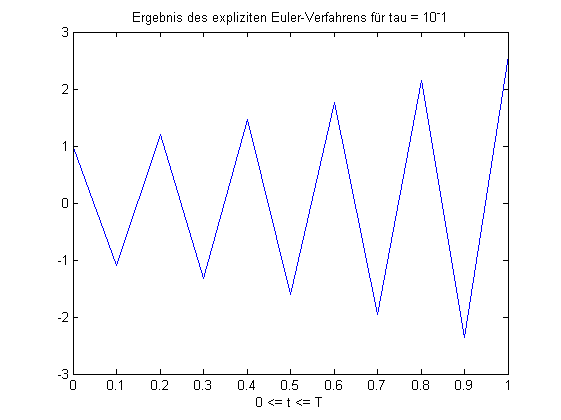
\includegraphics[scale=0.44]{exeuler1.png}
}
\subfigure[Plot des expliziten Euler-Verfahrens mit $\tau = 0.01$]{
	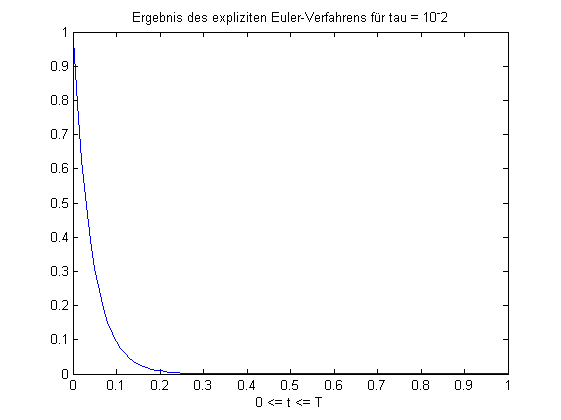
\includegraphics[scale=0.44]{exeuler2.png}
}
\subfigure[Plot des expliziten Euler-Verfahrens mit $\tau = 0.001$]{
	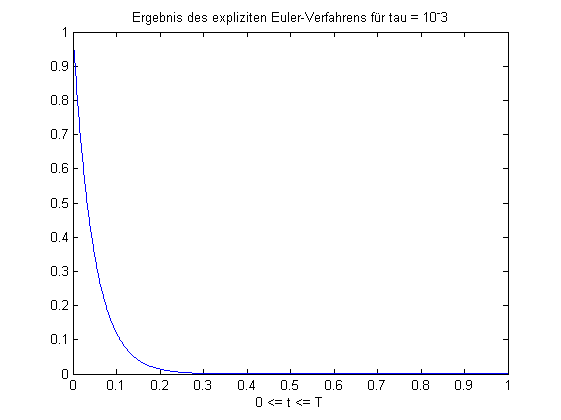
\includegraphics[scale=0.44]{exeuler3.png}
}
\end{figure}
\newpage
Im folgenden Programm wurde die Berechnung von $x_{k+1}$ durch Umstellen der Gleichung aus dem Skript erreicht.

\begin{lstlisting}[language=matlab, numbers=left]
function [ xk ] = impliciteuler(T, tau, lambda, f, x0 )
%impliciteuler berechnet das implizite Euler-Verfahren
%fuer das AWP x' = lambda*x+f, x(0) = x0 mit einem
%aequidistanten Gitter 0 = t0 < t1 < ... < tn = T

xk(1) = x0;
range = 0:tau:T; %% Gitter mit Abstand tau

%% Berechnungsvorschrift aus dem Skript in einer Schleife
for k = 1:size(range,2)-1,
    %% S bezeichnet die nach x_k (also xk(k)) umgestellte
    %% Gleichung der Berechnungsvorschrift
    S = (f(k*tau)*tau+xk(k))/(1-tau*lambda);
    xk(k+1) = S;
end
end
\end{lstlisting}

\begin{figure}[ht!]
\center
\subfigure[Plot des impliziten Euler-Verfahrens mit $\tau = 0.1$]{
	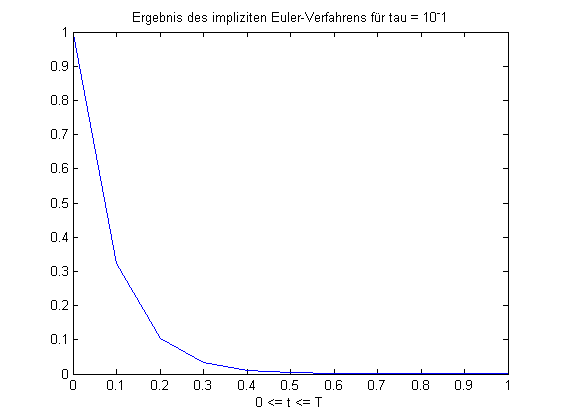
\includegraphics[scale=0.44]{imeuler1.png}
}
\subfigure[Plot des impliziten Euler-Verfahrens mit $\tau = 0.01$]{
	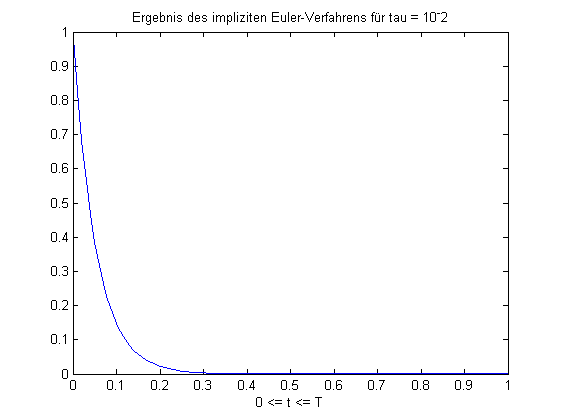
\includegraphics[scale=0.44]{imeuler2.png}
}
\subfigure[Plot des impliziten Euler-Verfahrens mit $\tau = 0.001$]{
	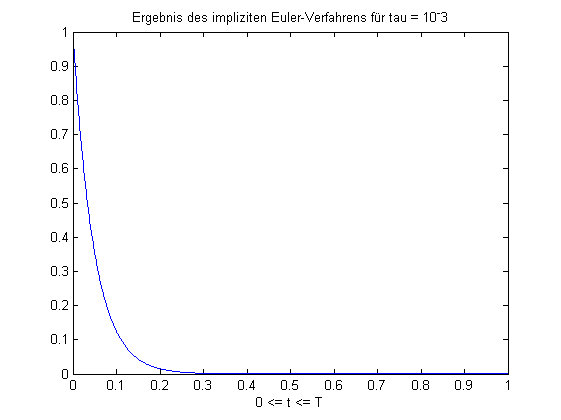
\includegraphics[scale=0.44]{imeuler3.png}
}
\end{figure}

Wir zu sehen ist, liefert das implizite Euler-Verfahren schon bei einer gröberen Schrittweite von $\tau = 0.1$ brauchbare Ergebnisse, wobei beim expliziten Euler-Verfahren bereits eine zehnfach genauere Schrittweite genutzt werden muss um sinnvolle Ergebnisse zu erhalten. Für feinere Gitter ($\tau \leq 0.01$) liefern beide Verfahren letztendlich gute Ergebnisse.
%% ------------------------------------------------------
%%                     AUFGABE 3
%% ------------------------------------------------------

%%\section*{Aufgabe 3}


\label{LastPage}

\end{document}
